\chapter{实证结果与分析}\label{chap:4}
\section{描述性统计}
主要变量的描述性统计结果如表\ref{tab:desc}所示。就保单而言,保额Coverage的均值为32.02万元,保费Premium的均值为1040元,保险标的购置价Price均值为52.64万元,发生赔付的保单赔付额平均约2.86万元。就气象数据而言,监测站点和保险标的的地理位置距离(distance)的均值为13.23公里,极端降水量均值401mm。就不同地区的指标而言,名义GDP增速的均值为17\%,保险深度平均79\%,保险密度平均236元。
% 表\ref{tab:corr}报告了主要变量的相关系数矩阵,变量相关系数极低,说明本文的实证研究结果不存在多重共线性。

\begin{table}[H]
    \caption{数据描述性统计}\label{tab:desc}
    \centering
    \begin{tabular}{lrrrrrr}
\toprule
 & 观测数 & 均值 & 标准差 & 最小值 & 中位数 & 最大值 \\
\midrule
Coverage & 741442 & 288407.75 & 318090.33 & 20092.78 & 192000.00 & 2991900.00 \\
Disaster & 741442 & 0.12 & 0.32 & 0 & 0 & 1 \\
Neighbor & 741442 & 0.04 & 0.20 & 0 & 0 & 1 \\
Post & 741442 & 0.88 & 0.33 & 0 & 1 & 1 \\
Price & 741442 & 47.26 & 49.75 & 0 & 30.50 & 371.07 \\
GDP & 741442 & 8422.33 & 11370.88 & 0.07 & 0.25 & 49110.27 \\
Density & 741442 & 224.97 & 152.41 & 39.47 & 183.02 & 821.75 \\
Penetration & 741442 & 0.78 & 0.17 & 0.45 & 0.79 & 1.20 \\
Prem\_before & 741442 & 0.03 & 0.16 & 0 & 0 & 1 \\
Claim & 741442 & 0 & 0.04 & 0 & 0 & 1 \\
Premium & 741442 & 1014.95 & 1025.45 & 10.20 & 650.00 & 5558.00 \\
累计赔付额 & 741442 & 33.77 & 2741.24 & 0 & 0 & 517183.53 \\
保费 & 741442 & 1014.95 & 1025.45 & 10.20 & 650.00 & 5558.00 \\
累计降水量 & 741442 & 1474.29 & 1090.56 & 0 & 1721.00 & 6203.00 \\
\bottomrule
\end{tabular}

\end{table}

图\ref{fig:dis}显示了标的与监测站距离分布,图\ref{fig:coverage}显示了标的保额分布,图\ref{fig:insurance}显示了保险标的保险起期分布,图\ref{fig:precip}显示了灾区家庭经历极端降水量分布。从图中可以看出,标的与监测站距离分布较近,保额分布呈现左偏分布,保险起期和灾区家庭经历极端降水量分布较为均匀。

\begin{figure}[H]
    \centering
    \begin{minipage}{0.48\linewidth}
        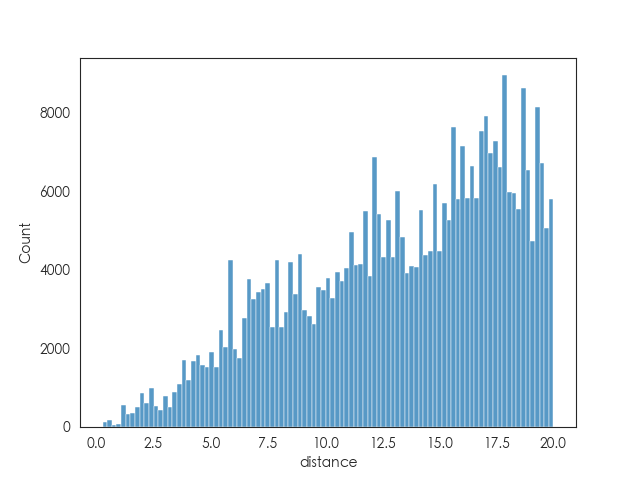
\includegraphics[width=\linewidth]{lib/img/olsdistance.png}
        \caption{标的与监测站距离分布}\label{fig:dis}
    \end{minipage}
    \begin{minipage}{0.48\linewidth}
        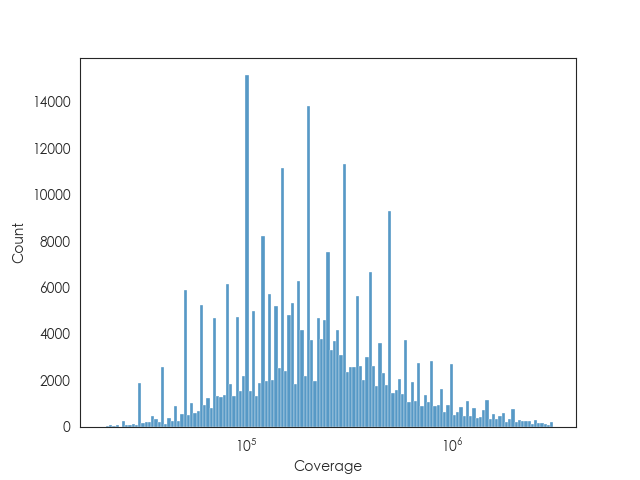
\includegraphics[width=\linewidth]{lib/img/coverage.png}
        \caption{标的保额分布}\label{fig:coverage}
    \end{minipage}
    \begin{minipage}{0.48\linewidth}
        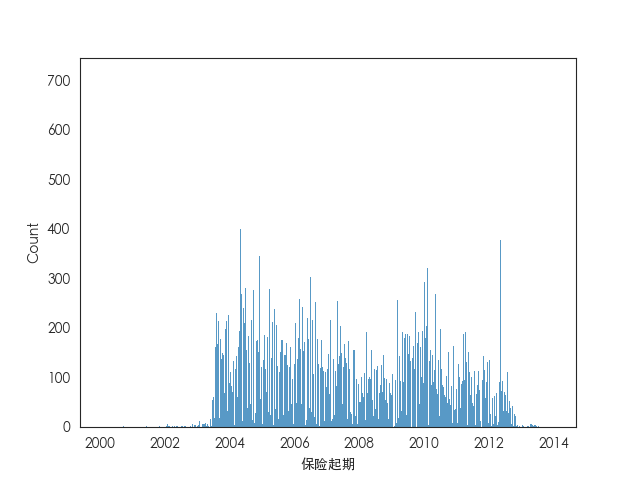
\includegraphics[width=\linewidth]{img/insurance.png}
        \caption{保险标的保险起期分布}\label{fig:insurance}
    \end{minipage}
    \begin{minipage}{0.48\linewidth}
        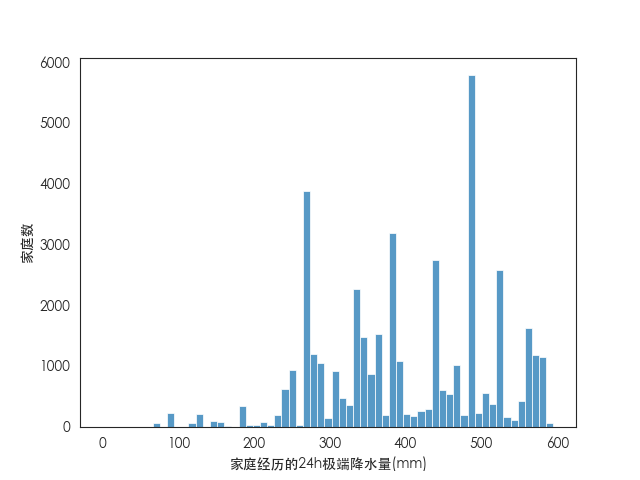
\includegraphics[width=\linewidth]{lib/img/precip.png}
        \caption{灾区家庭经历极端日降水量分布}\label{fig:precip}
    \end{minipage}
\end{figure}
% 截止2012年7月22日凌晨2时,北京全市平均降雨量164毫米,城区平均降雨量212毫米,降雨最大点在房山区河北镇,降雨量519毫米。
% \begin{table}[H]
%     \caption{变量之间相关性}\label{tab:corr}
%     \centering
%     \begin{tabular}{lrrrrrrr}
\toprule
 & Coverage & Disaster & Neighbor & Post & Prem\_before & Price & Area \\
\midrule
Coverage & 1.000000 & -0.003438 & 0.002232 & 0.006549 & 0.049063 & 0.195955 & -0.000131 \\
Disaster & -0.003438 & 1.000000 & -0.112619 & -0.199710 & -0.031179 & -0.027510 & -0.000619 \\
Neighbor & 0.002232 & -0.112619 & 1.000000 & -0.025723 & 0.004791 & 0.002799 & -0.000466 \\
Post & 0.006549 & -0.199710 & -0.025723 & 1.000000 & 0.014869 & 0.023873 & 0.000746 \\
Prem\_before & 0.049063 & -0.031179 & 0.004791 & 0.014869 & 1.000000 & 0.080722 & -0.000330 \\
Price & 0.195955 & -0.027510 & 0.002799 & 0.023873 & 0.080722 & 1.000000 & -0.000173 \\
Area & -0.000131 & -0.000619 & -0.000466 & 0.000746 & -0.000330 & -0.000173 & 1.000000 \\
\bottomrule
\end{tabular}


% \end{table}

\section{基准回归结果}
% \subsection{模型\ref{eq:OLS}:基础回归}
% 对于假设\ref{hyp:1},回归结果见表\ref{tab:ols}。

% \begin{table}[htbp]
%     \centering
%     \caption{OLS回归结果}\label{tab:ols}
%     
\begin{tabular}{@{\extracolsep{5pt}}lcc}
\\[-1.8ex]\hline
\hline \\[-1.8ex]
& \multicolumn{2}{c}{\textit{Dependent variable: log(Coverage)}} \
\cr \cline{2-3}
\\[-1.8ex] & (1) & (2) \\
\hline \\[-1.8ex]
 Area & & -0.000$^{}$ \\
& & (0.000) \\
 Intercept & 12.265$^{***}$ & 12.158$^{***}$ \\
& (0.004) & (0.003) \\
 Post & 0.100$^{***}$ & 0.071$^{***}$ \\
& (0.004) & (0.004) \\
 Prem\_before & & 0.670$^{***}$ \\
& & (0.008) \\
 Price & & 0.136$^{***}$ \\
& & (0.001) \\
\hline \\[-1.8ex]
 Observations & 414961 & 414961 \\
 $R^2$ & 0.001 & 0.171 \\
 Adjusted $R^2$ & 0.001 & 0.171 \\
 Residual Std. Error & 1.021 (df=414959) & 0.930 (df=414956) \\
 F Statistic & 584.020$^{***}$ (df=1; 414959) & 21392.415$^{***}$ (df=4; 414956) \\
\hline
\hline \\[-1.8ex]
\textit{Note:} & \multicolumn{2}{r}{$^{*}$p$<$0.1; $^{**}$p$<$0.05; $^{***}$p$<$0.01} \\
\end{tabular}

% \end{table}

\subsection{近灾区的DID回归}
对于假设\ref{hyp:3},回归结果见表\ref{tab:did1}。回归结果显示,在控制了其他变量之后,近灾区的交互项$\text{Neighbor}\times \text{Post}$的系数显著为正,这一结果验证了假设\ref{hyp:3},意味着在极端天气事件发生后,近灾区的保额提升了约24\%。近灾区居民由于接收到更丰富的信息,对极端天气事件的敏感度增强,因此他们的保险需求也相应增加。这种信息的丰富性可能来自于更直接的灾害经历、媒体报道、社区讨论等多种渠道,使得近灾区居民对灾害的潜在影响有了更深刻的认识。
\begin{table}[H]
    \centering
    \caption{实验组为近灾区的DID回归结果}\label{tab:did1}
    
\begin{tabular}{@{\extracolsep{5pt}}lcc}
\\[-1.8ex]\hline
\hline \\[-1.8ex]
& \multicolumn{2}{c}{\textit{Dependent variable: log(Coverage)}} \
\cr \cline{2-3}
\\[-1.8ex] & (1) & (2) \\
\hline \\[-1.8ex]
 Area & & -0.000$^{}$ \\
& & (0.000) \\
 Intercept & 12.164$^{***}$ & 12.067$^{***}$ \\
& (0.005) & (0.004) \\
 Neighbor & 0.227$^{***}$ & 0.224$^{***}$ \\
& (0.013) & (0.012) \\
 Neighbor:Post & 0.086$^{***}$ & 0.087$^{***}$ \\
& (0.015) & (0.014) \\
 Post & 0.095$^{***}$ & 0.068$^{***}$ \\
& (0.005) & (0.005) \\
 Prem\_before & & 0.542$^{***}$ \\
& & (0.008) \\
 Price & & 0.153$^{***}$ \\
& & (0.001) \\
\hline \\[-1.8ex]
 Observations & 455107 & 455107 \\
 $R^2$ & 0.006 & 0.136 \\
 Adjusted $R^2$ & 0.006 & 0.136 \\
 Residual Std. Error & 1.150 (df=455103) & 1.072 (df=455100) \\
 F Statistic & 961.465$^{***}$ (df=3; 455103) & 11948.789$^{***}$ (df=6; 455100) \\
\hline
\hline \\[-1.8ex]
\textit{Note:} & \multicolumn{2}{r}{$^{*}$p$<$0.1; $^{**}$p$<$0.05; $^{***}$p$<$0.01} \\
\end{tabular}

\end{table}

此外,当极端天气事件发生(即$\text{Post=1}$)时,不论家庭是否是否位于近灾区,家财险的保额整体上提高了约10\%。这一提升是显著为正,意味着在极端天气事件的影响下,家庭的风险感知得到了加强,从而增加了他们对家财险的需求。这一发现与假设\ref{hyp:3}的预期一致,即极端天气事件通过提高风险感知,导致家财险需求的提升。

控制变量方面,回归结果还表明,在家庭层面,保险标的的购置价每提升1\%导致保额平均提升0.34\%,家庭之前投保过会导致保额平均提升21\%。这两个变量的系数显著为正,与直觉相符,即价值较高的财和有保险购买历史的家庭更倾向于购买更高额度的保险。而在地区层面,GDP增速每增加1\%,家财险的保额整体上小幅提高约0.15\%,反应经济发展水平对保险需求的正向提升作用\citep{JJYJ200401002,arena2008does};而保险深度每提升1\%,家财险的保额整体上提高约0.66\%,反应保险市场的发展对保险需求的正向提升作用\citep{JRYJ200706018}。这两个变量的系数显著为正,与保险需求与经济发展水平、保险市场发展水平正相关的理论预期一致。

% 此外,DID回归结果还揭示了近灾区与远灾区之间的差异。近灾区的系数显著为正,表明与远灾区相比,近灾区的居民在灾害发生后购买的家财险保额提升了约22\%。这一差异可能源于近灾区居民对极端降水概率的主观判断更高,因此他们的风险感知也更强。这种强烈的风险感知可能促使他们购买更高额度的保险,以更好地保护自己的财产。

\subsection{灾区的DID回归}
对于假设\ref{hyp:2},回归结果见表\ref{tab:did2}。与表\ref{tab:did1}类似,该组也验证了假设\ref{hyp:3},即极端天气事件发生后购买家财险的保额提升约11\%。但是,交互项$\text{Disaster}\times \text{Post}$的系数为负,即灾区相对非灾区在受灾后反而降低了18\%保额,完全抵消了受灾后的11\%保额增加的影响,保额反而相对降低。其他控制变量的结果与表\ref{tab:did2}基本一致,保险标的的购置价、家庭之前投保过、GDP增速、保险深度等变量的系数符号与表\ref{tab:did1}一致,且显著性水平也基本一致。

\begin{table}[H]
    \centering
    \caption{实验组为灾区的DID回归结果}\label{tab:did2}
    
\begin{tabular}{@{\extracolsep{5pt}}lcc}
\\[-1.8ex]\hline
\hline \\[-1.8ex]
& \multicolumn{2}{c}{\textit{Dependent variable: log(Coverage)}} \
\cr \cline{2-3}
\\[-1.8ex] & (1) & (2) \\
\hline \\[-1.8ex]
 Area & & -0.000$^{}$ \\
& & (0.000) \\
 Disaster & 0.187$^{***}$ & 0.207$^{***}$ \\
& (0.009) & (0.008) \\
 Disaster:Post & -0.333$^{***}$ & -0.310$^{***}$ \\
& (0.011) & (0.010) \\
 Intercept & 12.164$^{***}$ & 12.071$^{***}$ \\
& (0.005) & (0.005) \\
 Post & 0.095$^{***}$ & 0.069$^{***}$ \\
& (0.005) & (0.005) \\
 Prem\_before & & 0.547$^{***}$ \\
& & (0.008) \\
 Price & & 0.144$^{***}$ \\
& & (0.001) \\
\hline \\[-1.8ex]
 Observations & 480733 & 480733 \\
 $R^2$ & 0.002 & 0.116 \\
 Adjusted $R^2$ & 0.002 & 0.116 \\
 Residual Std. Error & 1.163 (df=480729) & 1.095 (df=480726) \\
 F Statistic & 360.218$^{***}$ (df=3; 480729) & 10506.506$^{***}$ (df=6; 480726) \\
\hline
\hline \\[-1.8ex]
\textit{Note:} & \multicolumn{2}{r}{$^{*}$p$<$0.1; $^{**}$p$<$0.05; $^{***}$p$<$0.01} \\
\end{tabular}

\end{table}

\section{稳健性检验}
\subsection{平行趋势检验}

为了验证DID实证结果的稳健性,需要进行平行趋势检验。表\ref{tab:robust}展示了平行趋势检验的结果,并可视化如图\ref{fig:robust}。本文分别将实验组设置为灾区和近灾区($\text{Treat}=\text{Disaster}$以及$\text{Treat}=\text{Neighbor}$),对极端天气事件发生前四个季度的保额进行回归。回归结果显示交互项的系数都不显著,这表明在极端天气事件发生前,实验组和对照组的保额水平基本是平行的,满足平行趋势假设,可以通过DID方法来估计极端天气事件对家财险需求的影响。
% 唯一表现出显著性的部分是在灾区受灾前90天内(一个季度)的保额,这可能是因为20年一遇的极端降水往往是持续较久的,灾区居民达到20年一遇的门槛前已经开始感知到风险,从而提前购买了保险。

\begin{figure}[H]
    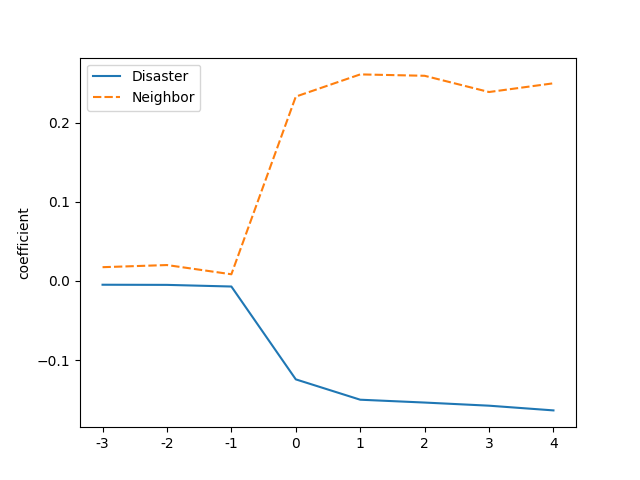
\includegraphics[width=\linewidth]{lib/img/robust.png}
    \caption{平行趋势检验}\label{fig:robust}
\end{figure}
\begin{table}[H]
    \centering
    % \renewcommand{\arraystretch}{0.8}
    \caption{平行趋势检验}\label{tab:robust}
    
\begin{tabular}{@{\extracolsep{5pt}}lcc}
\\[-1.8ex]\hline
\hline \\[-1.8ex]
& \multicolumn{2}{c}{\textit{Dependent variable: log(Coverage)}} \
\cr \cline{2-3}
\\[-1.8ex] & \multicolumn{1}{c}{Disaster} & \multicolumn{1}{c}{Neighbor}  \\
\\[-1.8ex] & (1) & (2) \\
\hline \\[-1.8ex]
 Treated:C(Quarter)[T.-1] & -0.007$^{}$ & 0.008$^{}$ \\
& (0.015) & (0.042) \\
 Treated:C(Quarter)[T.-2] & -0.005$^{}$ & 0.020$^{}$ \\
& (0.015) & (0.040) \\
 Treated:C(Quarter)[T.-3] & -0.005$^{}$ & 0.017$^{}$ \\
& (0.014) & (0.041) \\
 Treated:C(Quarter)[T.0] & -0.124$^{***}$ & 0.233$^{***}$ \\
& (0.011) & (0.030) \\
 Treated:C(Quarter)[T.1] & -0.150$^{***}$ & 0.261$^{***}$ \\
& (0.013) & (0.030) \\
 Treated:C(Quarter)[T.2] & -0.153$^{***}$ & 0.259$^{***}$ \\
& (0.013) & (0.030) \\
 Treated:C(Quarter)[T.3] & -0.157$^{***}$ & 0.238$^{***}$ \\
& (0.013) & (0.030) \\
 Treated:C(Quarter)[T.4] & -0.163$^{***}$ & 0.250$^{***}$ \\
& (0.013) & (0.030) \\
C(Quarter)[T.-1] & -0.006$^{}$ & -0.006$^{}$ \\
& (0.009) & (0.009) \\
 C(Quarter)[T.-2] & -0.004$^{}$ & -0.004$^{}$ \\
& (0.009) & (0.009) \\
 C(Quarter)[T.-3] & -0.002$^{}$ & -0.002$^{}$ \\
& (0.009) & (0.009) \\
 C(Quarter)[T.0] & 0.091$^{***}$ & 0.095$^{***}$ \\
& (0.007) & (0.007) \\
 C(Quarter)[T.1] & 0.096$^{***}$ & 0.099$^{***}$ \\
& (0.007) & (0.007) \\
 C(Quarter)[T.2] & 0.097$^{***}$ & 0.101$^{***}$ \\
& (0.007) & (0.007) \\
 C(Quarter)[T.3] & 0.096$^{***}$ & 0.100$^{***}$ \\
& (0.007) & (0.007) \\
 C(Quarter)[T.4] & 0.101$^{***}$ & 0.105$^{***}$ \\
& (0.007) & (0.007) \\
 Treated & -0.002$^{}$ & -0.211$^{***}$ \\
& (0.010) & (0.029) \\
 Controls & True & True \\
 Intercept & 10.986$^{***}$ & 11.042$^{***}$ \\
& (0.007) & (0.007) \\
\hline \\[-1.8ex]
 Observations & 709271 & 654504 \\
 $R^2$ & 0.385 & 0.364 \\
 Adjusted $R^2$ & 0.385 & 0.364 \\
 Residual Std. Error & 0.661  & 0.677  \\
 F Statistic & 21157.483$^{***}$  & 17827.292$^{***}$  \\
\hline
\hline \\[-1.8ex]
\textit{Note:} & \multicolumn{2}{r}{$^{*}$p$<$0.1; $^{**}$p$<$0.05; $^{***}$p$<$0.01} \\
\end{tabular}

\end{table}

\subsection{安慰剂检验}
为排除其他潜在政策和遗漏变量等对回归结果的干扰,本文参考\citet{CYJJ202104009}随机虚构处理组,将 Neighbor 和 Disaster 的 DID 随机分组分配重复 500 次,结果如图\ref{fig:randomtest}所示。随机分配结果的所有系数估计值大体呈均值为 0 的正态分布,说明实验结果不是由于其他潜在政策或遗漏变量引起的,而是由于极端天气事件的影响。
\begin{figure}[H]
    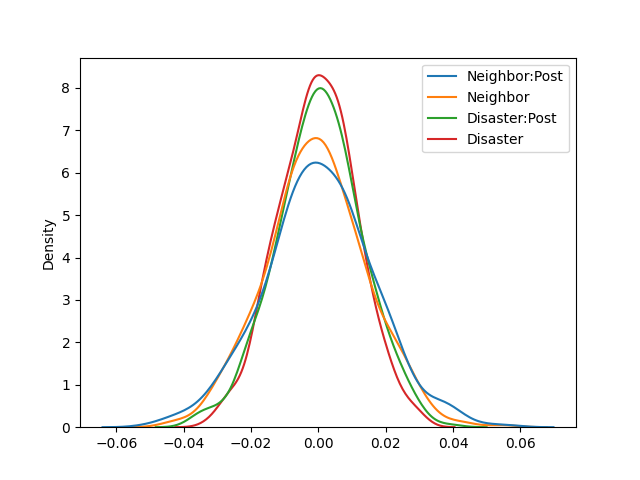
\includegraphics[width=\linewidth]{lib/img/randomtest.png}
    \caption{安慰剂检验}\label{fig:randomtest}
\end{figure}

\subsection{其他稳健性检验}

为保证基准回归结果的稳健性,本文还进行了以下稳健性检验:(1)(2)更换家财险需求的度量方式为保费Premium;(3)(4)/(5)(6)参考\citet{alok2020fund}分别将灾区距离上界从 20km 改为10km。回归结果如表\ref{tab:robustdid}所示。就回归结果而言,基本与基准回归结果一致,表明本文的实证结果是稳健的。这一结果进一步验证了极端天气事件通过增强家庭的风险感知,导致家财险需求的提升。
\begin{sidewaystable}[htbp]
    \centering
    \caption{稳健性检验回归结果}\label{tab:robustdid}
    
\begin{tabular}{@{\extracolsep{5pt}}lcccccc}
\\[-1.8ex]\hline
\hline \\[-1.8ex]
\\[-1.8ex] & \multicolumn{1}{c}{log(Premium)} & \multicolumn{1}{c}{log(Premium)} & \multicolumn{1}{c}{<30km} & \multicolumn{1}{c}{<30km} & \multicolumn{1}{c}{<10km} & \multicolumn{1}{c}{<10km}  \\
\\[-1.8ex] & (1) & (2) & (3) & (4) & (5) & (6) \\
\hline \\[-1.8ex]
 Area & 0.000$^{}$ & 0.000$^{}$ & 0.000$^{}$ & 0.000$^{}$ & 0.000$^{}$ & 0.000$^{}$ \\
& (0.000) & (0.000) & (0.000) & (0.000) & (0.000) & (0.000) \\
 Disaster & & -0.149$^{***}$ & & 0.187$^{***}$ & & 0.170$^{***}$ \\
& & (0.009) & & (0.006) & & (0.011) \\
 Disaster:Post & & -0.036$^{***}$ & & -0.207$^{***}$ & & -0.277$^{***}$ \\
& & (0.011) & & (0.007) & & (0.013) \\
 Intercept & 6.257$^{***}$ & 6.255$^{***}$ & 12.052$^{***}$ & 12.055$^{***}$ & 12.086$^{***}$ & 12.106$^{***}$ \\
& (0.005) & (0.005) & (0.003) & (0.003) & (0.006) & (0.006) \\
 Neighbor & 0.065$^{***}$ & & 0.222$^{***}$ & & 0.158$^{***}$ & \\
& (0.013) & & (0.012) & & (0.014) & \\
 Neighbor:Post & 0.024$^{}$ & & 0.150$^{***}$ & & 0.209$^{***}$ & \\
& (0.015) & & (0.013) & & (0.016) & \\
 Post & 0.097$^{***}$ & 0.097$^{***}$ & -0.000$^{}$ & -0.000$^{}$ & 0.085$^{***}$ & 0.098$^{***}$ \\
& (0.005) & (0.005) & (0.003) & (0.003) & (0.002) & (0.002) \\
 Prem\_before & -0.801$^{***}$ & -0.785$^{***}$ & 0.574$^{***}$ & 0.576$^{***}$ & 0.386$^{***}$ & 0.395$^{***}$ \\
& (0.009) & (0.009) & (0.006) & (0.006) & (0.009) & (0.010) \\
 Price & 0.084$^{***}$ & 0.086$^{***}$ & 0.184$^{***}$ & 0.178$^{***}$ & 0.238$^{***}$ & 0.198$^{***}$ \\
& (0.001) & (0.001) & (0.001) & (0.001) & (0.001) & (0.001) \\
\hline \\[-1.8ex]
 Observations & 408439 & 433025 & 853757 & 939148 & 270762 & 277046 \\
 $R^2$ & 0.041 & 0.038 & 0.150 & 0.131 & 0.190 & 0.146 \\
 Adjusted $R^2$ & 0.041 & 0.038 & 0.150 & 0.131 & 0.190 & 0.146 \\
 Residual Std. Error & 1.138  & 1.143  & 1.076  & 1.098  & 1.022  & 1.065  \\
 F Statistic & 2885.524$^{***}$  & 2880.383$^{***}$  & 25027.608$^{***}$  & 23637.295$^{***}$  & 10588.824$^{***}$  & 7863.860$^{***}$  \\
\hline
\hline \\[-1.8ex]
\textit{Note:} & \multicolumn{6}{r}{$^{*}$p$<$0.1; $^{**}$p$<$0.05; $^{***}$p$<$0.01} \\
\end{tabular}

\end{sidewaystable}

具体而言,表\ref{tab:robustdid}的模型(1)(2)显示,当极端天气事件发生后,家庭的保费整体上提高了约5\%。这一提升是显著为正,意味着在极端天气事件的影响下,家庭的风险感知得到了加强,从而增加了他们对家财险的需求。这一发现与假设\ref{hyp:3}的预期一致,即极端天气事件通过提高风险感知,导致家财险需求的提升。但灾区交互项的系数为负,表明灾区的保费在受灾后反而降低了约16\%,近灾区则提升了约57\%,与假设\ref{hyp:3}、假设\ref{hyp:2}一致。

就更改距离而言,模型(3)(4)/(5)(6)分别更改灾区受灾半径的上界至10km/30km,整体而言并不会改变实证结果,同样显示出灾区灾后保额购买减少约10-15\%、近灾区保额购买提升25-30\%,表明本文的实证结果是稳健的。

\section{异质性分析}
\subsection{地区异质性}
在探讨极端天气事件对不同地区影响的差异性时,本文首先关注了地区对此类事件的反应是否存在显著的地域性差异。基于东部沿海地区频繁遭受降水事件的影响,居民可能因多次面对风险而逐渐形成了对此类风险的适应性预期。正如台风路径上的企业对自然灾害的反应效率提升\citep{0Do},频繁的降水可能为他们累积了经验,降低了对极端天气的敏感度\citep{陈思柳2021不同决策情境下的损失厌恶效应差异}。
相反,在干旱少雨的西部地区,由于降水事件较为罕见,由于降水相对较少对极端降水风险的敏感度不足,这可能导致他们在面对极端天气时的反应与东部地区存在显著差异。

为了验证这一假设,本研究根据国家统计局的划分标准,将样本划分为东部、中部和西部三个地区,并分别进行了回归分析。回归结果如表\ref{tab:het_geo}所示,基本与表\ref{tab:did1}和表\ref{tab:did2}一致。东部和中部地区在遭受极端降水事件后,灾区交互项系数为负,表明保险金额有所下降,而在近灾区,保险金额的增长更为显著。

\begin{sidewaystable}[htbp]
    \centering
    \caption{分地区回归结果}\label{tab:het_geo}
    
\begin{tabular}{@{\extracolsep{5pt}}lcccccc}
\\[-1.8ex]\hline
\hline \\[-1.8ex]
& \multicolumn{6}{c}{\textit{Dependent variable: log(Coverage)}} \
\cr \cline{2-7}
\\[-1.8ex] & \multicolumn{1}{c}{East} & \multicolumn{1}{c}{Middle} & \multicolumn{1}{c}{West} & \multicolumn{1}{c}{East} & \multicolumn{1}{c}{Middle} & \multicolumn{1}{c}{West}  \\
\\[-1.8ex] & (1) & (2) & (3) & (4) & (5) & (6) \\
\hline \\[-1.8ex]
 Disaster & -0.090$^{***}$ & 0.054$^{***}$ & -0.159$^{***}$ & & & \\
& (0.006) & (0.008) & (0.006) & & & \\
 Disaster:Post & -0.121$^{***}$ & -0.136$^{***}$ & 0.123$^{***}$ & & & \\
& (0.007) & (0.009) & (0.008) & & & \\
 Neighbor & & & & -0.233$^{***}$ & -0.136$^{***}$ & -0.490$^{***}$ \\
& & & & (0.016) & (0.018) & (0.129) \\
 Neighbor:Post & & & & 0.246$^{***}$ & 0.052$^{***}$ & 0.570$^{***}$ \\
& & & & (0.017) & (0.019) & (0.129) \\
 Post & 0.065$^{***}$ & 0.036$^{***}$ & -0.171$^{***}$ & 0.065$^{***}$ & 0.037$^{***}$ & -0.172$^{***}$ \\
& (0.004) & (0.004) & (0.004) & (0.004) & (0.004) & (0.004) \\
%  Prem\_before & 0.185$^{***}$ & 0.107$^{***}$ & 0.067$^{***}$ & 0.174$^{***}$ & 0.106$^{***}$ & 0.071$^{***}$ \\
% & (0.006) & (0.030) & (0.016) & (0.006) & (0.034) & (0.016) \\
%  log(GDP) & 0.000$^{}$ & 0.000$^{}$ & -0.000$^{}$ & 0.000$^{}$ & 0.000$^{}$ & -0.000$^{}$ \\
% & (0.000) & (0.000) & (0.000) & (0.000) & (0.000) & (0.000) \\
%  log(Penetration) & 0.906$^{***}$ & 0.029$^{***}$ & 0.071$^{***}$ & 0.909$^{***}$ & 0.027$^{***}$ & 0.116$^{***}$ \\
% & (0.005) & (0.007) & (0.005) & (0.005) & (0.008) & (0.005) \\
%  log(Price) & 0.312$^{***}$ & 0.684$^{***}$ & 0.848$^{***}$ & 0.296$^{***}$ & 0.672$^{***}$ & 0.852$^{***}$ \\
% & (0.001) & (0.002) & (0.001) & (0.001) & (0.002) & (0.002) \\
Intercept & 11.386$^{***}$ & 9.757$^{***}$ & 9.331$^{***}$ & 11.444$^{***}$ & 9.793$^{***}$ & 9.298$^{***}$ \\
& (0.005) & (0.006) & (0.007) & (0.006) & (0.007) & (0.007) \\
Controls & True & True & True & True & True & True \\
\hline \\[-1.8ex]
 Observations & 481063 & 123513 & 104695 & 450350 & 107232 & 96922 \\
 $R^2$ & 0.333 & 0.593 & 0.764 & 0.314 & 0.585 & 0.774 \\
 Adjusted $R^2$ & 0.333 & 0.592 & 0.764 & 0.314 & 0.585 & 0.774 \\
 Residual Std. Error & 0.704  & 0.439  & 0.375  & 0.718  & 0.447  & 0.364  \\
 F Statistic & 34345.705$^{***}$  & 25654.772$^{***}$  & 48356.638$^{***}$  & 29449.242$^{***}$  & 21634.683$^{***}$  & 47450.879$^{***}$  \\
    Year FE & True & True & True & True & True & True \\
\hline
\hline \\[-1.8ex]
\textit{Note:} & \multicolumn{6}{r}{$^{*}$p$<$0.1; $^{**}$p$<$0.05; $^{***}$p$<$0.01} \\
\end{tabular}

\end{sidewaystable}

然而,在西部地区,极端降水事件冲击导致灾区的交互项系数则显著为正,这与东部和中部地区的情况形成了鲜明对比。原因可能有两方面:一方面由于西部地区极端降水事件虽然也是20年一遇,但由于西部通常干旱,极端降水事件打破其心理预期幅度较大,如图\ref{fig:rainings}所示,因此导致灾区和近灾区居民反应更剧烈,导致远灾区和近灾区的显著性不高,同时回归的数值也相对较小。
另一方面,西部地区居民在灾难前对极端降水风险的敏感度较低,很难唤醒保险需求,容易低估了极端天气发生的概率\citep{tversky1973availability},导致保险覆盖不足,如图\ref{fig:covbyregion}。因此,在巨灾发生后,他们可能有补充保障的动机,这反映在灾区交互项系数显著为正上。

\begin{figure}[H]
    \centering
    \begin{minipage}{0.48\linewidth}
        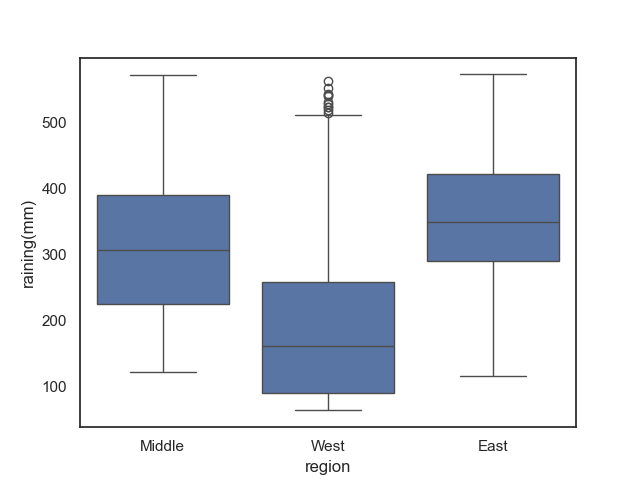
\includegraphics[width=\linewidth]{lib/img/rainings.png}
        \caption{分地区20年一遇极端降水量框线图}\label{fig:rainings}
    \end{minipage}
    \begin{minipage}{0.48\linewidth}
        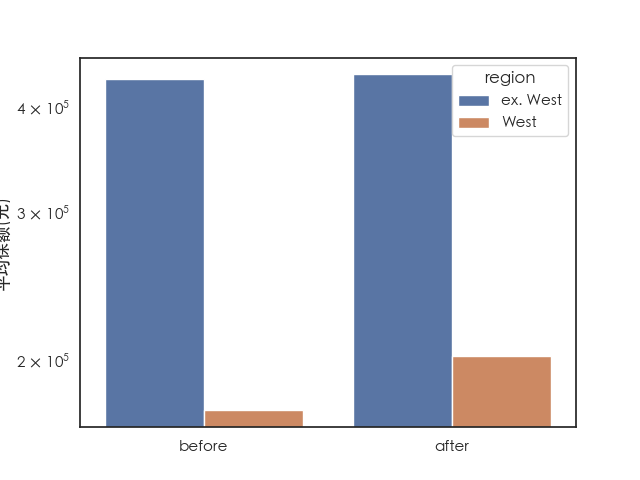
\includegraphics[width=\linewidth]{lib/img/covbyregion.png}
        \caption{不同地区在极端降水发生前后保额}\label{fig:covbyregion}
    \end{minipage}
\end{figure}

综上所述,本研究的结果揭示了不同地区对极端天气事件的反应确实存在显著的地域性差异。这种差异可能源于地区间对极端天气风险感知程度的不同,进而导致了不同的保险需求水平。但总的来说,这一发现与假设\ref{hyp:3}的预期保持一致,即极端天气事件本质上是通过提高风险感知,导致家财险需求的增加

\subsection{时间异质性}
2008年是一个特殊年份,在经济领域发生了金融危机,在自然领域发生了汶川地震。本文以2008年为界,将样本最丰富的时间段分割为2003-2008年和2009-2013年两段,以探讨家庭感知到巨大风险之后面对极端天气事件时反应是否有差异。表\ref{tab:het_time}显示了时间异质性分析结果,也与表\ref{tab:did1}和表\ref{tab:did2}基本一致,即表现为极端天气事件发生后近灾区购买家财险的保额普遍提升,但灾区提升相对有限。

\begin{table}[H]
    \centering
    \caption{分时间回归结果}\label{tab:het_time}
    
\begin{tabular}{@{\extracolsep{5pt}}lcccc}
\\[-1.8ex]\hline
\hline \\[-1.8ex]
& \multicolumn{4}{c}{\textit{Dependent variable: log(Coverage)}} \
\cr \cline{2-5}
\\[-1.8ex] & \multicolumn{1}{c}{2003-2008} & \multicolumn{1}{c}{2009-2013} & \multicolumn{1}{c}{2003-2008} & \multicolumn{1}{c}{2009-2013}  \\
\\[-1.8ex] & (1) & (2) & (3) & (4) \\
\hline \\[-1.8ex]
 Disaster & 0.017$^{*}$ & -0.013$^{}$ & & \\
& (0.010) & (0.014) & & \\
 Disaster:Post & -0.170$^{***}$ & -0.089$^{***}$ & & \\
& (0.012) & (0.017) & & \\
 Intercept & 11.821$^{***}$ & 12.417$^{***}$ & 11.859$^{***}$ & 12.542$^{***}$ \\
& (0.006) & (0.006) & (0.005) & (0.007) \\
 Neighbor & & & 0.440$^{***}$ & -0.297$^{***}$ \\
& & & (0.012) & (0.043) \\
 Neighbor:Post & & & 0.032$^{*}$ & 0.211$^{***}$ \\
& & & (0.014) & (0.045) \\
 Post & 0.072$^{***}$ & 0.087$^{***}$ & 0.086$^{***}$ & 0.033$^{***}$ \\
& (0.006) & (0.007) & (0.006) & (0.008) \\
%  Prem\_before & 0.196$^{***}$ & 0.784$^{***}$ & 0.336$^{***}$ & 0.768$^{***}$ \\
% & (0.011) & (0.011) & (0.010) & (0.012) \\
%  Price & 0.187$^{***}$ & 0.113$^{***}$ & 0.166$^{***}$ & 0.125$^{***}$ \\
% & (0.001) & (0.001) & (0.001) & (0.001) \\
\hline \\[-1.8ex]
 Observations & 268828 & 191588 & 301508 & 139476 \\
 $R^2$ & 0.102 & 0.156 & 0.119 & 0.183 \\
 Adjusted $R^2$ & 0.102 & 0.156 & 0.119 & 0.183 \\
 Residual Std. Error & 0.982  & 1.058  & 0.998  & 1.045  \\
 F Statistic & 6122.243$^{***}$  & 7057.294$^{***}$  & 8131.866$^{***}$  & 6243.412$^{***}$  \\
\hline
\hline \\[-1.8ex]
\textit{Note:} & \multicolumn{4}{r}{$^{*}$p$<$0.1; $^{**}$p$<$0.05; $^{***}$p$<$0.01} \\
\end{tabular}

\end{table}

值得注意的是,交互项在2008年后显示出很强的正向提升,这可能是由于汶川地震及金融危机使得家庭对于风险感知更为明显,居民对家庭所在周边的环境更为关注,对极端天气事件的风险感知提升,从而增加了对更高保额家财险的需求。

\subsection{保险标的价值异质性}

保险标的价值可能对人们的保险购买行为有影响,价值越高的家庭财产在风险意识提升后,保险需求增加的幅度可能更大。本文采用保额的大小作为保险标的价值的代理变量,将样本平均分为低、中、高三组,进行回归分析。其中低保额组的保额在3.95万-14万元,中保额组的保额在14万-30万元之间,高保额组的保额在30万-168万元。回归结果如表\ref{tab:het_cov}所示,近灾区的交互项显示出随保额递增的趋势,说明保险标的价值越高,近灾区的保险需求增加越明显,这可能是由于家庭对高价值的家庭财产的损失可能更为敏感,因此保险需求增加的幅度更大。
而对于灾区的交互项系数显示出随保额递减的趋势,高保额组可能由于居民认为短期内不会再次受灾或是受资金影响,保险需求减少,部分因此转为低保额组,导致减少幅度相对于高保额组更轻。
\begin{sidewaystable}[ht]
    \centering
    \caption{按保额大小异质性分析}\label{tab:het_cov}
    
\begin{tabular}{@{\extracolsep{5pt}}lcccccc}
\\[-1.8ex]\hline
\hline \\[-1.8ex]
& \multicolumn{6}{c}{\textit{Dependent variable: log(Coverage)}} \
\cr \cline{2-7}
\\[-1.8ex] & \multicolumn{1}{c}{low} & \multicolumn{1}{c}{mid} & \multicolumn{1}{c}{high} & \multicolumn{1}{c}{low} & \multicolumn{1}{c}{mid} & \multicolumn{1}{c}{high}  \\
\\[-1.8ex] & (1) & (2) & (3) & (4) & (5) & (6) \\
\hline \\[-1.8ex]
 Disaster & -0.013$^{***}$ & 0.017$^{***}$ & -0.066$^{***}$ & & & \\
& (0.003) & (0.002) & (0.004) & & & \\
 Disaster:Post & -0.003$^{}$ & -0.033$^{***}$ & -0.117$^{***}$ & & & \\
& (0.004) & (0.003) & (0.005) & & & \\
 Neighbor & & & & 0.096$^{***}$ & -0.060$^{***}$ & -0.115$^{***}$ \\
& & & & (0.007) & (0.006) & (0.023) \\
 Neighbor:Post & & & & -0.099$^{***}$ & 0.064$^{***}$ & 0.138$^{***}$ \\
& & & & (0.008) & (0.006) & (0.024) \\
 Post & 0.017$^{***}$ & 0.017$^{***}$ & 0.009$^{***}$ & 0.018$^{***}$ & 0.017$^{***}$ & 0.008$^{***}$ \\
& (0.002) & (0.002) & (0.003) & (0.002) & (0.002) & (0.003) \\
%  Prem\_before & 0.117$^{***}$ & 0.028$^{***}$ & 0.015$^{***}$ & 0.114$^{***}$ & 0.029$^{***}$ & 0.008$^{**}$ \\
% & (0.005) & (0.003) & (0.004) & (0.005) & (0.002) & (0.004) \\
%  log(GDP) & 0.000$^{**}$ & -0.000$^{}$ & 0.000$^{}$ & 0.000$^{**}$ & -0.000$^{}$ & 0.000$^{*}$ \\
% & (0.000) & (0.000) & (0.000) & (0.000) & (0.000) & (0.000) \\
%  log(Penetration) & 0.123$^{***}$ & 0.083$^{***}$ & 0.158$^{***}$ & 0.126$^{***}$ & 0.077$^{***}$ & 0.146$^{***}$ \\
% & (0.003) & (0.002) & (0.003) & (0.003) & (0.002) & (0.004) \\
%  log(Price) & 0.086$^{***}$ & 0.028$^{***}$ & 0.071$^{***}$ & 0.080$^{***}$ & 0.025$^{***}$ & 0.067$^{***}$ \\
% & (0.001) & (0.000) & (0.001) & (0.001) & (0.000) & (0.001) \\
Intercept & 11.207$^{***}$ & 12.063$^{***}$ & 12.668$^{***}$ & 11.226$^{***}$ & 12.071$^{***}$ & 12.685$^{***}$ \\
& (0.003) & (0.002) & (0.004) & (0.003) & (0.002) & (0.004) \\
Controls & True & True & True & True & True & True \\
\hline \\[-1.8ex]
 Observations & 232914 & 217205 & 214095 & 211102 & 199829 & 200904 \\
 $R^2$ & 0.072 & 0.033 & 0.081 & 0.068 & 0.030 & 0.074 \\
 Adjusted $R^2$ & 0.072 & 0.033 & 0.081 & 0.068 & 0.030 & 0.074 \\
 Residual Std. Error & 0.284  & 0.182  & 0.311  & 0.284  & 0.183  & 0.316  \\
 F Statistic & 2570.208$^{***}$  & 1053.810$^{***}$  & 2706.248$^{***}$  & 2205.864$^{***}$  & 893.130$^{***}$  & 2291.168$^{***}$  \\
 Year FE & True & True & True & True & True & True \\
\hline
\hline \\[-1.8ex]
\textit{Note:} & \multicolumn{6}{r}{$^{*}$p$<$0.1; $^{**}$p$<$0.05; $^{***}$p$<$0.01} \\
\end{tabular}

\end{sidewaystable}

\subsection{城市级别异质性}

我国仍面临一定程度的城乡二元化的问题,地级市居民和县区居民在收入、教育、医疗、社会保障等方面存在较大差异,这可能导致他们对极端天气事件的风险感知程度不同,进而影响他们的保险需求。本文将样本分为地级市(包含各直辖市各区)和县区两组,进行回归分析。回归结果如表\ref{tab:het_rur}所示。居民与此前DID回归(见表\ref{tab:did1}及表\ref{tab:did2})基本一致,但是县区灾区和近灾区的交互项绝对值相比于地级市更低。灾区可能是由于县区居民与农业关系更密切,对极端天气事件的风险感知程度更高,并且县区基础设施较差、受二十年一遇降水的冲击可能更严重。近灾区可能是由于县区居民的经济水平和家庭财产保险覆盖率相对较低\citep{falco2014crop,胡新艳2021气候变化,TJLT202108007},因此对家财险的接受程度更低,县区家财险投保样本仅占总样本的约1/3。

\begin{table}[ht]
    \centering
    \caption{按城市级别异质性分析}\label{tab:het_rur}
    
\begin{tabular}{@{\extracolsep{5pt}}lcccc}
\\[-1.8ex]\hline
\hline \\[-1.8ex]
& \multicolumn{4}{c}{\textit{Dependent variable: log(Coverage)}} \
\cr \cline{2-5}
\\[-1.8ex] & \multicolumn{1}{c}{农村} & \multicolumn{1}{c}{农村} & \multicolumn{1}{c}{城市} & \multicolumn{1}{c}{城市}  \\
\\[-1.8ex] & (1) & (2) & (3) & (4) \\
\hline \\[-1.8ex]
 Disaster & -0.022$^{*}$ & & 0.283$^{***}$ & \\
& (0.013) & & (0.011) & \\
 Disaster:Post & 0.115$^{***}$ & & -0.543$^{***}$ & \\
& (0.016) & & (0.014) & \\
 Intercept & 12.094$^{***}$ & 12.094$^{***}$ & 12.206$^{***}$ & 12.206$^{***}$ \\
& (0.007) & (0.007) & (0.006) & (0.006) \\
 Neighbor & & -0.120$^{***}$ & & 0.358$^{***}$ \\
& & (0.021) & & (0.016) \\
 Neighbor:Post & & 0.143$^{***}$ & & 0.106$^{***}$ \\
& & (0.024) & & (0.018) \\
 Post & -0.022$^{***}$ & -0.022$^{***}$ & 0.140$^{***}$ & 0.140$^{***}$ \\
& (0.008) & (0.007) & (0.007) & (0.007) \\
\hline \\[-1.8ex]
 Observations & 160810 & 148210 & 317651 & 304242 \\
 $R^2$ & 0.001 & 0.000 & 0.005 & 0.013 \\
 Adjusted $R^2$ & 0.001 & 0.000 & 0.005 & 0.013 \\
 Residual Std. Error & 1.027  & 1.017  & 1.216  & 1.195  \\
 F Statistic & 40.420$^{***}$  & 12.639$^{***}$  & 554.450$^{***}$  & 1304.637$^{***}$  \\
\hline
\hline \\[-1.8ex]
\textit{Note:} & \multicolumn{4}{r}{$^{*}$p$<$0.1; $^{**}$p$<$0.05; $^{***}$p$<$0.01} \\
\end{tabular}

\end{table}
